\documentclass[a4paper]{report}

%--- stock basic pkgs --------------------------------
\usepackage[T1]{fontenc}
\usepackage[utf8]{inputenc}
\usepackage{lmodern}
\usepackage{geometry}
\usepackage{amsmath ,amsthm ,amssymb}
\usepackage{fancyhdr} % Required for custom headers
\usepackage{extramarks} % Required for headers and footers
\usepackage{float}
\usepackage[english]{babel}
\usepackage{fancyhdr}
\usepackage{verbatim}
\usepackage{tikz}
\usepackage{showframe}
\usepackage{graphics}

%--- installed basic pkgs -------------------------------
\usepackage{apacite}
\usepackage{comment}
\usepackage[all]{nowidow}
\usepackage{enumitem}
\usepackage{csquotes}
\usepackage{outlines}
\usepackage{bibentry}  %Required to insert full citation in text
\usepackage{pdfpages}
\usepackage{lastpage}  % Required to determine the last page for the footer
\usepackage{everypage} % Required for watermarks
\usepackage{draftwatermark}
\SetWatermarkLightness{0.90}
\SetWatermarkScale{4}



%% LaTeX Preamble - Font choices
%% Each block selects new math, roman (serif), sans serif, and typewriter fonts.
%% Delete or comment out all but one to make your choice.

% Fourier for math | Utopia (scaled) for rm | Helvetica for ss | Latin Modern for tt
\usepackage{fourier} % math & rm
\usepackage[scaled=0.875]{helvet} % ss
\renewcommand{\ttdefault}{lmtt} %tt

% Latin Modern (similar to CM with more characters)
\usepackage{lmodern} % math, rm, ss, tt
\usepackage[T1]{fontenc}

% Palatino for rm and math | Helvetica for ss | Courier for tt
\usepackage{mathpazo} % math & rm
\linespread{1.05}        % Palatino needs more leading (space between lines)
\usepackage[scaled]{helvet} % ss
\usepackage{courier} % tt
\normalfont
\usepackage[T1]{fontenc}

% Euler for math | Palatino for rm | Helvetica for ss | Courier for tt
\renewcommand{\rmdefault}{ppl} % rm
\linespread{1.05}        % Palatino needs more leading
\usepackage[scaled]{helvet} % ss
\usepackage{courier} % tt
\usepackage{euler} % math
%\usepackage{eulervm} % a better implementation of the euler package (not in gwTeX)
\normalfont
\usepackage[T1]{fontenc}

% Times for rm and math | Helvetica for ss | Courier for tt
\usepackage{mathptmx} % rm & math
\usepackage[scaled=0.90]{helvet} % ss
\usepackage{courier} % tt
\normalfont
\usepackage[T1]{fontenc}

% !! COMMERICAL FONT !! Lucida Bright (w/expert package)
\usepackage[T1]{fontenc}
\usepackage[expert,vargreek,altbullet]{lucidabr}

%% END Font choices



%%%%%%%%%%%%%%%%%%%%%%
%% THE TIPS %%%%%%%%%%
%%%%%%%%%%%%%%%%%%%%%%


%-----------fancy math ---------
\
\[
\left.
\begin{aligned}
  &\sqrt{{dX_{1}}^{2} + {dX_{2}}^{2} + {dX_{3}}^{2}} \\
  &\qquad
  \begin{aligned}
  &= \left(1 + \frac{\kappa}{8\pi} \int \frac{\sigma\, dV_{0}}{r}\right)
     \sqrt{{dx_{1}}^{2} + {dx_{2}}^{2} + {dx_{3}}^{2}}, \\
dT &= \left(1 - \frac{\kappa}{8\pi} \int \frac{\sigma\, dV_{0}}{r}\right) dl.
\end{aligned}
\end{aligned}
\right\}
\]


%----using multicolumn for complex tables----------

% problem ==> goes outside margins

\begin{tabular}{|*{18}{c|}}  % repeats {c|} 18 times
\hline
\multicolumn{9}{|c}{k-means clustering} & \multicolumn{9}{|c|}{Fuzzy c-means clustering} \\ \hline
\multicolumn{3}{|c}{50 clusters} & \multicolumn{3}{|c}{60 clusters} & \multicolumn{3}{|c}{70 clusters} & 
\multicolumn{3}{|c}{50 clusters} & \multicolumn{3}{|c}{60 clusters} & \multicolumn{3}{|c|}{70 clusters} \\ \hline 
CJ & HT & SVD &CJ & HT & SVD &CJ & HT & SVD &CJ & HT & SVD &CJ & HT & SVD &CJ & HT & SVD \\ \hline
 & & & & & & & & & & & & & & & & &  \\ \hline
\end{tabular}


% fix ==> use p{}

\begin{longtable}{p{1cm} p{1cm} p{1cm} p{1cm} p{1cm}}
\caption{Review of two lesson plans based on the television show, "Friends"}\\
\toprule
\multicolumn{1}{c}{X} & \multicolumn{2}{|c}{k-means clustering} & \multicolumn{2}{|c}{k-means clustering} \\
x & y & z & w & T\\
\toprule

\midrule

\bottomrule
\end{longtable}


% fix it again
\begin{longtable}{*{8}{p{1cm}}}  % repeats {c|} 18 times
%\begin{longtable}{p{2cm} p{3cm} p{3cm}}
\caption{Review of two lesson plans based on the television show, "Friends"}\\
\toprule
\multicolumn{2}{c}{x} & \multicolumn{3}{|c}{k-means} & \multicolumn{3}{|c}{clustering} \\
CJ & HT & SVD & CJ & HT & SVD & CJ & HT \\
\toprule

\midrule

\bottomrule
\end{longtable}







%--------------- Fix image position ----

\usepackage{float}

...

\begin{figure}[H]
\centering
\includegraphics{slike/visina8}
\caption{Write some caption here}\label{visina8}
\end{figure}




% ----------Lists with various labels for sequences -----------------


\begin{enumerate}[label=\arabic*.]
\item Create a pleasant and supportive class atmosphere
\item Make the curriculum and teaching materials relevant to the students.
\item  Make learning stimulating and enjoyable by increasing attractiveness of the tasks.
\item  Build learners' confidence by providing regular encouragement.
\item  Build students' confidence in their skill by teaching them various learning strategies.
\item Increase students' motivation by actively promoting learning autonomy.
\end{enumerate}





%----------- date -----------------------

\today

\date{\today}


%------------ graphics in outline --------------------

\begin{outline}[enumerate]
\1 \textbf{Install Git 2.18.0}
\2 Go to the \enquote{Git for Windows} site (\href{https://gitforwindows.org/}{left-click here})
\3 Click on the \enquote{Download} button to download, \enquote{Git-2.18.0-64-bit.exe}
\3 Run the \enquote{Git-2.18.0-64-bit.exe} installer accepting defaults EXCEPT
\4 Check daily for Git Windows updates
\4[] \includegraphics[scale = 0.30]{graphics/Screenshot1.png}
\4 Use Notepadd++ as Git's default editor (We'll install Notepad++ in a moment.)

\end{outline}




%------------- change bullets in itemize -------------------

\renewcommand{\labelitemi}{$\bullet$}
\renewcommand{\labelitemii}{$\cdot$}
\renewcommand{\labelitemiii}{$\diamond$}
\renewcommand{\labelitemiv}{$\ast$}


\usepackage{enumitem}
\begin{itemize}[label={$\bullet$}]
\end {itemize}

\begin{itemize}[label={$\cdot$}]
\end {itemize}

\begin{itemize}[label={$\diamond$}]
\end {itemize}

\begin{itemize}[label={$\ast$}]
\end {itemize}

\begin{itemize}[label={--}]
\end {itemize}




%--------- inverted Spanish question mark, exclamation mark -------------------
Use a tick mark:

?`
!` 


%---------- ellipsis -----------------------
$\ldots$


%------- section symbol section sign --------------

\S


%---------- aspect ratio graphics ---------------

\includegraphics[width=6in, height=6in, keepaspectratio]{graphics/Rplot01}
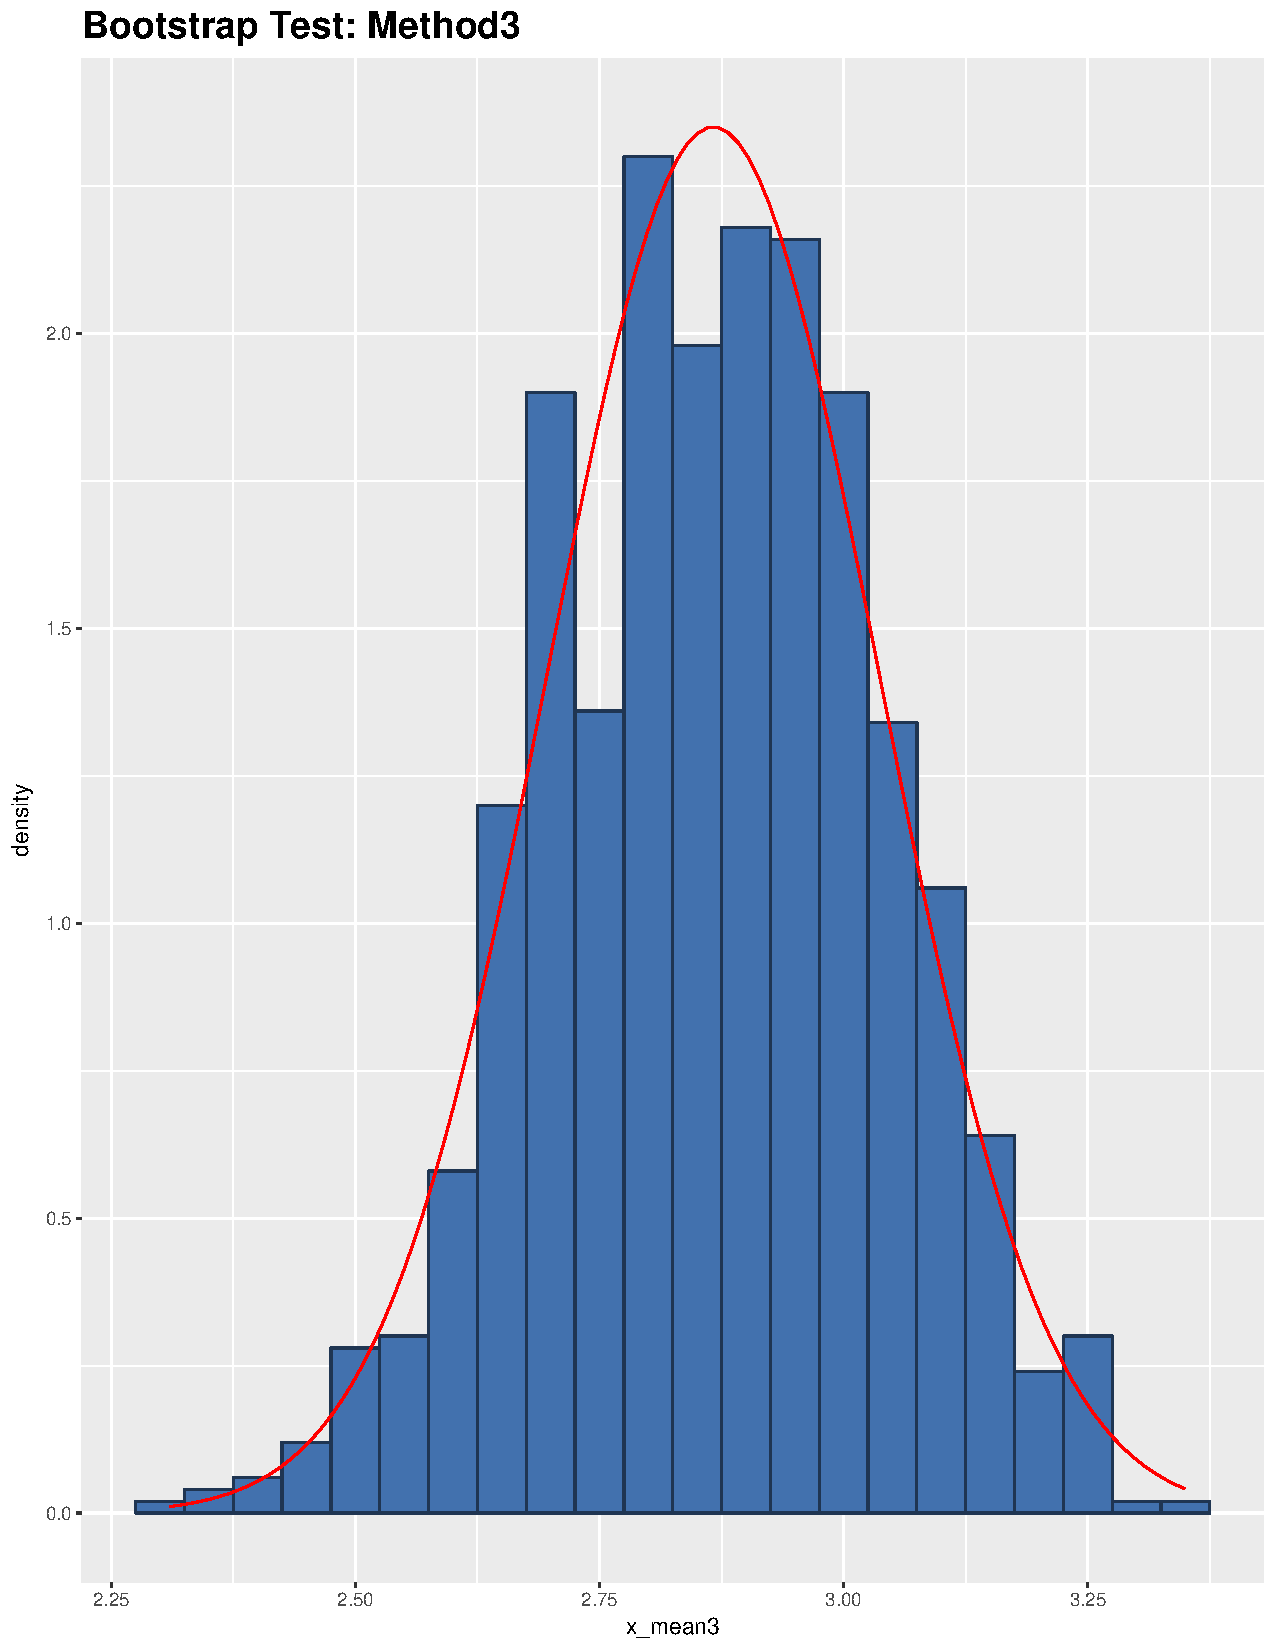
\includegraphics[width=\paperwidth, height=\paperheight, keepaspectratio]{graphics/Rplot1}



%-------prevent page break for lists/enumerate ---------------
\begin{samepage}
\begin{enumerate}
  \item \textbf{The output delivered by Upwork is, at best, misleading and incomplete.} FPL should be very cautious about using this service to provide statistical analysis as the basis for generating client projections. 
  \item \textbf{The method of resampling should continue to be used until better statistical models and approaches are developed for FPL.} The use of resampling coupled with the BCA confidence interval is a valid statistical approach for obtaining statistics from FPL datasets.
  \item \textbf{The FPL practice of quota sampling can produce a representative sample given a set of assumptions woven into a logic model.} A logic model, based on sound survey design principles, can provide justification for continued quota sampling by FPL.
\end{enumerate}
\end{samepage}





%--------- wrap text in table ------------------------------------
Use p{width} for your column specifiers instead of l/r/c.

\begin{tabular}{p{1cm}p{3cm}}



%----------- indent paragraph --------------------

\newenvironment{myindentpar}[1]%
   {\begin{list}{}%
       {\setlength{\leftmargin}{#1}}%
           \item[]%
   }
     {\end{list}}

%	#to use in doc
%\begin{myindentpar}{1em}
%text
%\end{myindentpar}

%----------- footnotes in letter --------------------------------

\usepackage[hang,flushmargin,multiple]{footmisc} 
 \footcite{priest_program_2001}\textsuperscript{,}\footcite{worthen_program_1990}.

%----------- table with bullets ----------------------
\begin{table}[!htbp]
  \caption{Some important theoretical considerations for social program evaluation.} 
  \label{tab:bm3} 
\begin{tabular} {p{4cm}p{10cm}}
\toprule
Theoretical Component &  Consideration\\
\midrule
  Social Programming  & \\
  & \begin{itemize}
    \item Know the political and historical origins of a program, its internal structure, governance, and funding; the ways in which is implemented; its context; available leverage points
    \item Attend to the internal structure and functioning of a program as well as to its external context and change potentials
  \end{itemize} \\
  
  Knowledge Construction  & \\
  & \begin{itemize}
    \item Significant difficulties plague all ontologies and epistomologies; no method is routinely feasible and unbiased
    \item Claiming to construct knowledge that is special or authoritative requires that the theory of knowledge construction used be made explicit
    \item The effect of interventions depends on initial conditions; internal validity is not causal; the authority of the randomized experiment must be questioned (Cronbach)
  \end{itemize} \\
  
  Value  & \\
  & \begin{itemize}
    \item Social programs are themselves not value-free; they involve decisions about expenditure of social resources
    \item Data do not speak for themselves but are interpreted in terms that invoke values
    \item Evaluation is assumed to serve the \enquote{public good}; rarely is this assumption explicated; most evaluations implicitly use descriptive valuing
    \item Descriptive valuing (judgment of program worth based on stakeholder values); there is no claim of one set of values being better than another; no training in ethics required
    \item Prescriptive valuing (judgment of program worth based on comparison to an ethical philosophy); claims primacy of one set of values; training in ethics required
    \item What variables are studied depends on the evaluator's conception (mental model) of the system; the mental model is shaped by personal ethics    
  \end{itemize} \\
  
    Use  & \\
  & \begin{itemize}
    \item Evaluation results may be used instrumentally (for direct decision making), conceptually (for increasing the depth and breadth of what social programs do), or persuasively (for advocacy)
    \item Evaluation results have both short-term and long-term effects
    \item Evaluation results are rarely compelling relative to the interests and ideologies of stakeholders; stakeholders usually regard scientific input as minor in decision making
    \item Evaluation results often threaten entrenched interests
    \item Evaluation results rarely enter public debates as uncontested nuggets of truth
  \end{itemize} \\
  
 \bottomrule
\end{tabular}
\end{table}


%----------- set table column width ----------------
\begin{table}[!htbp]
  \caption{Some important theoretical considerations for social program evaluation.} 
  \label{tab:bm3} 
\begin{tabular}{p{4cm}p{10cm}}
\toprule
Theoretical Component &  Consideration\\
\midrule
  Social Programming  & \\
  & Evaluators must know the political and historical origins of a program, its internal structure, governance, and funding; \\
  & the ways in which is implemented; its context; available leverage points \\
  
 \bottomrule
\end{tabular}
\end{table}
 

% -------------URLs in pdf; hyperreferences --------------------------
https://tex.stackexchange.com/questions/107832/how-to-create-internet-link-in-pdf

\usepackage{hyperref}
\hypersetup{
    colorlinks=true,
    linkcolor=blue,
    filecolor=magenta,      
    urlcolor=cyan,
}
\begin{document} 
    For more information about 'TikZ' click on the following link: 
    \href{http://www.texample.net/tikz/resources/}{Tex Example Site}
\end{document}



%  ------------ insert minipage w/ graphics and a boxed border -----------------------------
\fbox{
\begin{minipage} [t][][c]{0.80\linewidth}
\includegraphics[scale=0.10]{graphics/PBEM_logo.jpg}
\textbf{Portland Bureau of Emergency Management}\\
\textit{Disaster risk reduction through leadership and coordination.}\\

Following a major disaster, first responders who provide fire and medical services will not be able to meet the demand for these services. Factors such as number of victims, communication failures and road blockages will prevent people from accessing emergency services that they have come to expect at a moment's notice through 911. People will have to rely on each other for help in order to meet their immediate life saving and life sustaining needs. \\

\includegraphics[scale=0.25]{graphics/NET_logo.jpg}
\textbf{Portland Neighborhood Emergency Team Program}\\
 When you volunteer for Portland NET ...\\
...you will actively participate in important activities that make a difference.\\
...you will have the opportunity to better yourself personally and professionally.\\
...you will make a difference in the lives of others.\\
...you will make connections with others.
 \end{minipage}
}







%----------- Spanish exclamation mark --------------
A question/exclamation mark followed by a backtick (?`) 
produces the inverted character: ¿


%------------ blank lines --------------------
\par is a TeX primitive and is the same as a blank line (except in special environments such as verbatim where the usual rules don't apply). It ends horizontal mode, causes TeX to break the horizontal text into lines placed on the current vertical list, and exercises the page breaker which may possibly cause the next page to be shipped out.

\\ is different in almost every respect. It is a macro not a primitive, and its definition changes wildly in almost every LaTeX definition. The definition in normal text, a center environment a flushleft environment and a table are all different.





%-------- checkmark------------------------------------
$\checkmark$


% ----- no page number in bibliography -------------------

%----------------------------------------------------------------------------------------
%	(old)
%----------------------------------------------------------------------------------------
\clearpage 
\renewcommand{\thepage}{}
\bibliographystyle{/usr/local/share/texmf/tex/latex/apacite/apacite}
\bibliography{/home/bruce/Desktop/BibTex/My_Library_20170125}




%------- spacing between sections ------------------------

\usepackage{titlesec}
\titlespacing{command}{left spacing}{before spacing}{after spacing}[right]

\titlespacing\section{0pt}{12pt plus 4pt minus 2pt}{0pt plus 2pt minus 2pt}
\titlespacing\subsection{0pt}{12pt plus 4pt minus 2pt}{0pt plus 2pt minus 2pt}
\titlespacing\subsubsection{0pt}{12pt plus 4pt minus 2pt}{0pt plus 2pt minus 2pt}

\titlespacing*{\section}{0pt}{0.50\baselineskip}{0.25\baselineskip}

From the titlesec package

% spacing: how to read {12pt plus 4pt minus 2pt}
%           12pt is what we would like the spacing to be
%           plus 4pt means that TeX can stretch it by at most 4pt
%           minus 2pt means that TeX can shrink it by at most 2pt
%       This is one example of the concept of, 'glue', in TeX





%---- line numbers in pdf ----------------------------

\usepackage{lineno}
\usepackage{lipsum}
\begin{document}
    \linenumbers
    \lipsum
\end{document}


% --------- UTF-8 encoding not valid -------------------
 Use this sequence 
 
\usepackage[utf8]{inputenc}
\usepackage{csquotes}
\usepackage[T1]{fontenc}


%%------- gantt charts ---------------------

\usepackage{pgfgantt}

\begin{ganttchart}[
vgrid, 
hgrid,
bar/.append style={fill=green!20, rounded corners=2pt}
]{1}{24}
\gantttitle{2017}{12}
\gantttitle{2018}{12} \\
\ganttgroup{Group 1}{1}{3} \\
\ganttbar{Task 1}{1}{2} \\
\ganttbar{Task 2}{2}{2} \\
\ganttgroup{Group 2}{4}{12} \\
\ganttbar[bar height=.6]{Task 2}{4}{10} \\
\ganttmilestone{Milestone 1}{11}
\end{ganttchart}



\begin{ganttchart}[
vgrid,
title/.append style={fill=blue!40},
title label font=\sffamily\bfseries\color{white},
bar/.append style={fill=black, rounded corners=1pt},
bar left shift=.15,
bar right shift=-.15,
bar top shift=.4,
bar height=.2,
bar label font=\footnotesize,
milestone label font={\footnotesize \itshape \bfseries},
milestone/.append style={fill=green},
group left shift=0,
group right shift=0,
group peaks tip position=0,
group peaks height=.4
]{1}{24}
\gantttitle{Year 1}{12}
\gantttitle{Year 2}{12} \\
\ganttbar{Literature Review}{1}{3} \\
\ganttbar{Data Collection }{2}{5} \\
\ganttbar{Functions and Functionals}{3}{7}\\
\ganttbar{Translation to C\#}{4}{8}\\
\ganttbar{Unit Tests 1}{7}{12} \\
\ganttbar{LANDIS-II Interface}{11}{16}\\
\ganttbar{Unit Tests 2}{15}{19}\\
\ganttbar{Validations}{18}{23}\\
\ganttmilestone{AgroEV Release}{24}
\end{ganttchart}


% ------  adjusting captions ----------------------------

For global effect
\usepackage[width=.75\textwidth]{caption}


For local effect only in current environment:
\usepackage{caption}
\captionsetup{width=.75\textwidth}



%------ extra vertical space ----------------------


This is the line. \\~\\

Adds more space before this line


%------- isotopes and chemistry ------------------------

\usepackage{mhchem}

 \ce{^{227}_{90}Th+}    %\ce is chemical equation


%---- begin numbering (enumerate list) at different digit ----------------------- 

You can change the counter named enumi, like this:

\begin{enumerate}
  \setcounter{enumi}{4}
  \item fifth element
\end{enumerate}



%------- citations in natbib-----------

\usepackage[natbibapa]{apacite}

\shortcites{zhao_drought-induced_2010, hoegh-guldberg_impact_2010, eigenbrod_impact_2011, dodds_human_2013, rogers_facing_2008, lobell_climate_2011, wada_global_2010, tilman_forecasting_2001, tilman_agricultural_2002, zhao_drought-induced_2010}\citep{hoegh-guldberg_impact_2010, eigenbrod_impact_2011, dodds_human_2013, rogers_facing_2008, lobell_climate_2011, wada_global_2010, tilman_forecasting_2001, tilman_agricultural_2002, zhao_drought-induced_2010}.



% ---------- suppresses paragraph indentation ----------------------

\noindent 


%---- no section numbers ----------------------------------
\subsection*{Top Priority}


%------ new line ------------------------------------
\newline

%------- reduce space between items in a list ----------------------
 \begin{itemize}  
 \itemsep -2pt % reduce space between items
 \item Developed four "user friendly" forecasting  systems each of which produces 18 to 139 individual reports. 
 \item   Developed or improved almost all IFPS programs used for financial reports. 
\end{itemize}



%------- sloppy paragraphs -------------------------

\begin{sloppypar}
\noindent \texttt{The current model of industrial agriculture jeopardizes sustainability and the long-term delivery of ecosystem goods and services.}\\
\end{sloppypar}

%---- resize bullets in bullet list -------------------------------

% standard
\begin{itemize}
\item One
\item Two
\end{itemize}


% very small
\renewcommand\labelitemi{$\cdot$}  %add in \usepackage area of doc

\begin{itemize}
\item One
\item Two
\end{itemize}

% medium 
\renewcommand\labelitemi{{\boldmath$\cdot$}}  %add in \usepackage area of doc

\begin{itemize}
\item One
\item Two
\end{itemize}



%---------the regulatory "section" symbol -----------------------------

\usepackage{xspace}
\let\OldS\S
\renewcommand{\S}{\OldS\xspace}

\S 13

\OldS 13

%%-------- nested lists ----------------------------------------------------------

\documentclass{article}
\usepackage[shortlabels]{enumitem}

\begin{document}
\begin{enumerate}[1)]
  \item Level 1
  \begin{enumerate}[A)]
    \item sublevel A
    \begin{enumerate}[i)]
      \item sublevel i
       \begin{enumerate}[a)]
         \item sublevel a
       \end{enumerate}
    \end{enumerate}
  \end{enumerate}




%--------- fix position table/figure -------------------------------------------------
\begin{table}[!htbp]
\begin{figure}[!htbp]



%------ large doc organization: table of contents, list of figures, list of tables ---------------

\tableofcontents
\clearpage
\listoffigures
\clearpage
\listoftables


%--- accents and special characters ----------------------
%http://tex.stackexchange.com/questions/8857/how-to-type-special-accented-letters-in-latex

use \'e



%--- check installed pkgs ------------------------
as of 20160621
$ cd /usr/local/share/texmf/tex/latex
$ ls 

abstract    csquotes        everypage  nicefrac   sectsty         titlesec
adjustbox   cuposter        floatrow   nowidow    smartdiagram    units
apacite     datetime2       lastpage   outlines   standalone      wrapfig
bibentry    draftwatermark  lettrine   paralist   texMemo         xstring
changepage  enumitem        lipsum     preview    textpos
comment     etoolbox        multirow   psuposter  threeparttable




%-----comment out large sections----------------------------------------
\usepackage{comment}

\begin{comment}

\end{comment}


%---- using lipsum -----------------------------------------
\usepackage{lipsum}

\lipsum[1] % Dummy abstract text
\lipsum[2] % Dummy abstract text
\lipsum[3] % Dummy abstract text
\lipsum[4] % Dummy abstract text



%------line spacing; mathpazo and Palatino font ---------------------------------------------------------

	#use Palatino for the text and the Pazo fonts for math; a common combo
\usepackage[sc]{mathpazo}	%sc=small caps
\linespread{1.05}  
\usepackage[T1]{fontenc}
\usepackage[utf8]{inputenc}
\usepackage{microtype} % Slightly tweak font spacing for aesthetics





% ----- set margins ----------------------------------
	#use package 'geometry'
\documentclass[12pt,english]{article}
\usepackage[letterpaper,bindingoffset=0.2in,%
            left=1in,right=1in,top=1in,bottom=1in,%
            footskip=.25in]{geometry}
            
\usepackage[scale=0.90]{geometry}
\usepackage[left=0.5in, right=0.5in, top=0.5in, bottom=0.5in]{geometry}
\usepackage[margin=0.5in]{geometry}           

\usepackage[hmarginratio=1:1,top=32mm]{geometry} % Document margins


	#In the middle of the document if you want to change the margins use
\newgeometry{left=0.8in,right=0.8in,top=1in,bottom=1in}


%---- centering text on a page ----------------------------------------
\newpage
\vspace*{5cm}	%adjust as needed
\begin{center}
\LARGE \textbf{Appendix}
\end{center}

%----- text outside margins; using typewriter font overruns margins ------------------------

	# put the font inside sloppypar 
\begin{sloppypar}
\texttt{Element 3. The dynamic 'managed mosaic' created by the traditional agricultural practices of the Lowland Mayan in the Yucatan Peninsula during their Classical Period is an example of an as-yet, unexplained natural experiment in agricultural-ecological mutualism.}\\
\end{sloppypar}


% ---- the \textxx{} commands --------------
http://tex.stackexchange.com/questions/5008/when-to-use-bold-italics-small-caps-typewriter-etc

The visual \textXX commands will change 3 axes of the text: shape, family and weight.

    The shape axis covers: \textup, \textit, \textsc and \textsl
    The family axis covers: \textrm, \textsf, \texttt
    The weight axis covers: \textbf, \textmd




% --- continue numbered list after an insert ---------------
\usepackage{enumitem}
\begin{enumerate}
\item First item.
\item Second item.
\end{enumerate}
Text.
\begin{enumerate}[resume]
\item Third item
\end{enumerate}


%---- quotes ------------
\usepackage{csquotes}

\enquote{ text }
\enquote*{ text }

%------longtable caption width goes the full textwidth----------------------
\usepackage{etoolbox}
\setlength{\LTcapwidth}{=6.95in}	 



%---------place a full citation in text ---------------------------
\usepackage{natbib}
\usepackage{bibentry}
 
\begin{document}

\nobibliography*
\bibentry{higgins_why_2014}\\
\bibentry{camerer_progress_1997}

\newpage
\bibliography{/home/bmarron//Desktop/BibTex/My_Library_20160621}
\bibliographystyle{apalike}
\end{document}


%--------outlines-------------------------------------------
\usepackage{outlines}
\usepackage{enumitem}
\setenumerate[1]{label=\Roman*.}
\setenumerate[2]{label=\Alph*.}
\setenumerate[3]{label=\arabic*.}
\setenumerate[4]{label=\alph*.}

%% OR

\setenumerate[1]{label=\arabic*.}
\setenumerate[2]{label=\alph*.}
\setenumerate[3]{label=\roman*.}
\setenumerate[4]{label=$\bullet$}

in document,
\begin{outline}[enumerate]
\1 Level 1 
\2 Level 2
\3 Level 3
\4 Level 4
\end{outline}


%----------derivatives - limits - sums - integrals -----------------------

	#partials
\[ \frac{\partial u}{\partial t}
= h^2 \left( \frac{\partial^2 u}{\partial x^2}
+ \frac{\partial^2 u}{\partial y^2}
+ \frac{\partial^2 u}{\partial z^2} \right) \]

	#limits
\lim_{x\to +\infty} , \inf_{x > s}
\[ \lim_{x \to +\infty} \frac{3x^2 +7x^3}{x^2 +5x^4} = 3.\]


	#sums
\[ \sum_{k=1}^n k^2 = \frac{1}{2} n (n+1).\]

	#integrals
\[ \int_a^b f(x)\,dx.\]

\[ \int_0^{+\infty} x^n e^{-x} \,dx = n!.\]

\[ \int \cos \theta \,d\theta = \sin \theta.\]

\[ \int_{x^2 + y^2 \leq R^2} f(x,y)\,dx\,dy = \int_{\theta=0}^{2\pi} \int_{r=0}^R
f(r\cos\theta,r\sin\theta) r\,dr\,d\theta.\]

\[ \int_0^R \frac{2x\,dx}{1+x^2} = \log(1+R^2).\]

\[ \int_0^1 \! \int_0^1 x^2 y^2\,dx\,dy.\]

\[ \int \!\!\! \int_D f(x,y)\,dx\,dy.\]



In non-relativistic wave mechanics, the wave function
$\psi(\mathbf{r},t)$ of a particle satisfies the
\emph{Schr\"{o}dinger Wave Equation}
\[ i\hbar\frac{\partial \psi}{\partial t}
= \frac{-\hbar^2}{2m} \left(
\frac{\partial^2}{\partial x^2}
+ \frac{\partial^2}{\partial y^2}
+ \frac{\partial^2}{\partial z^2}
\right) \psi + V \psi.\]
It is customary to normalize the wave equation by
demanding that
\[ \int \!\!\! \int \!\!\! \int_{\textbf{R}^3}
\left| \psi(\mathbf{r},0) \right|^2\,dx\,dy\,dz = 1.\]
A simple calculation using the Schr\"{o}dinger wave
equation shows that
\[ \frac{d}{dt} \int \!\!\! \int \!\!\! \int_{\textbf{R}^3}
\left| \psi(\mathbf{r},t) \right|^2\,dx\,dy\,dz = 0,\]
and hence
\[ \int \!\!\! \int \!\!\! \int_{\textbf{R}^3}
\left| \psi(\mathbf{r},t) \right|^2\,dx\,dy\,dz = 1\]
for all times~$t$. If we normalize the wave function in this
way then, for any (measurable) subset~$V$ of $\textbf{R}^3$
and time~$t$,
\[ \int \!\!\! \int \!\!\! \int_V
\left| \psi(\mathbf{r},t) \right|^2\,dx\,dy\,dz\]
represents the probability that the particle is to be found
within the region~$V$ at time~$t$.





%---- delete small space ------------
\!


%--------headers ----------------------------------
\setlength{\headheight}{22pt}
\pagestyle{fancy}

\begin{document}
\rhead{\footnotesize \thepage\ of 2 }

%----Import .pdf graphics (e.g., from R) ------
	#export graphic as pdf (for OpenOffice export as jpg)
	#insert complete pdfs into current doc (or slides)
	
\usepackage{pdfpages}
\includepdf[pages={1-10}]{Experiment1b.pdf}
\includepdf[pages={1-10},pagecommand={},width=\textwidth]{file.pdf}

% ----Import graphics from GoogleDrive shared docs ----------

	a.
	#copy figure/graphic
	#open LibreOffice and paste graphic here
	#save graphic as .png file to Desktop
	#manipulate in GIMP, if needed
	#import as graphic to LaTex


%-------Import .txt like it was typed in LaTex ------------

	# a Tex primitive
\begingroup
\obeylines
\input{/home/bmarron//Desktop/Spring_2014/STAT_505_Fountain/HW1/RandWalk1_Model.txt}
\endgroup



%----- matrices ---------------------------

The \emph{characteristic polynomial} $\chi(\lambda)$ of the
$3 \times 3$~matrix
\[ \left( \begin{array}{ccc}
a & b & c \\
d & e & f \\
g & h & i \end{array} \right)\]
is given by the formula
\[ \chi(\lambda) = \left| \begin{array}{ccc}
\lambda - a & -b & -c \\
-d & \lambda - e & -f \\
-g & -h & \lambda - i \end{array} \right|.\]



%-------reference figure cite figure label tables in a big doc; table reference------------------

	#in the text of the doc
... Figure~\ref{fig:bm1} ....

	#somewhere after the text
\begin{figure}
	\begin{center}
		\includegraphics[scale=.60]{graphics/ws_map3.jpeg}
		\caption{Location of grid points for HadGEM2 weather data.}
		\label{fig:bm1}
	\end{center}
\end{figure}


%-------referencing tables in a big doc; figure reference ------------------
	#in the text of the doc
 ... Table~\ref{tab:bm1} ......
 
 
 % ------- big, three-part tables with footnotes ------------------
 
 \usepackage{threeparttable}
 
 \begin{table}
\footnotesize
  \begin{threeparttable}[b]
    \caption{The current input variables, functions, functionals, and output metrics for AgroEV.}
      \label{tab:bm1}
      \centering\captionsetup{width=.75\textwidth}
      \setlength{\tabcolsep}{2 mm}    
    \begin{tabular}{ll}
    \hline \hline \\[-1.8ex]
     Object &  Definition \\
    \hline \\[-1.8ex]
    Inputs \tnote{1} & $a_1$ = Cell area ($m^2$) \\
    & $a_2$ = Plant species and life history data (spp.)\\
    & $a_3$ = Basic soil edaphics (cell) \\
    & $a_4$ = Basic climate data (he cell) \\
    & $b_1$ = Biomass: below ground soil fungi and soil bacteria ($\mu g / g$ / cell)\\
    & $b_2$ = Concentrations of $Na^{+}, \ Ca^{2+}, \ Mg^{2+}$ (meq/mL / cell)\\
    & $b_3$ = Cation exchange capacity (meq/100g dirt / cell)\\
    & $b_4$ = Depth to a compacted soil layer (or bedrock) (m / cell)\\
    & $b_5$ = Applied N (kg/cell)\\
    & $b_6$ = Applied P (kg/cell)\\
    & $b_7$ = Applied C (kg/cell)\\
    & $b_8$ = Root architecture (spp.)\\ 
    Internal LANDIS-II & \\
    Data (D-Series) \tnote{2} & $D_1$ = Species and age (cohort/cell/timestep) \\
    & $D_2$ = Net primary productivity (cell/timestep)\\
    & $D_3$ = Biomass: aboveground cohorts (cell/timestep)\\
    Internal AgroEV & \\
    Data (F-Series) \tnote{3} & $F_1$ = Sodium adsorption ratio (cell/timestep) = $f(b_2)$ = $ {\frac {Na^{+}}{\sqrt {{\tfrac {1}{2}}({Ca^{2+}+Mg^{2+}})}}}$ \\
    & $F_2$ = Root density and dimensionality (cell/timestep) \\
    & \ \ \ \ \ = $f(a_1 \dots a_4, b_1, b_3 \dots b_8, D_1 \dots D_3, F_1)$\\
    & $F_3$ = Shannon diversity indices (aboveground) (cell/timestep) = $ f(D_1)$ \\
    Internal AgroEV & \\
    Data (G-series) \tnote{3} & $G_1$ = Rhizospheric density and dimensionality (cell/timestep) = $f(F_1 \dots F_3)$  \\
    & $G_2$ = Diversity of carbon inputs: root exudates (cell/timestep) = $f(F_3)$ \\
    & $G_3$ = Diversity of carbon inputs: litter (cell/timestep) = $f(b_7, D_1, F_3)$ \\
    & $G_4$ = Biomass: below ground soil fungi and soil bacteria (cell/timestep) \\
    & \ \ \ \ \ = $ f(D_1 \dots D_3, F_2, G_1 \dots G_3) $ \\
    & $G_5$ = Ratio of soil fungi-to-bacteria  (cell/timestep)= $ f(G_1 \dots G_4)$ \\
    Internal AgroEV & \\
    Data (H-series) \tnote{3} & $H_1$ = Joint prob. dist. of soil food web classes (cell/timestep) = $ f(G_1 \dots G_5)$ \\
    & $H_2$ = Marginal prob. dist. of a soil food web class (cell/timestep) = $ f(H_1)$ \\
    Output AgroEV & \\
    Data (O-Series) \tnote{4} & $O_1$ = Soil cation exchange capacity (cell/timestep) = $f(b_3, H_1)$ \\
    & $O_2$ = Rate of topsoil formation (O-horizon and A-horizon)  = $f(H_1)$ \\
    & $O_3$ = Shannon diversity indices (below ground) (cell/timestep) = $ f(H_1)$ \\
    & $O_4$ = Productivity index (cell/timestep) = $ \frac{Biomass \ from \ NPP}{Biomass \ extracted}$ = $ f(D_2, D_3, H_1)$ \\
	\hline \\[-1.8ex]
    \end{tabular}
    \begin{tablenotes}
    \footnotesize 
    \item [1] a-series are standard LANDIS-II inputs; b-series are new, AgroEV inputs 
    \item [2] D-series are time series data internally generated by LANDIS-II 
    \item [3] F-series, G-series, and H-series are new time series data internally generated by AgroEV
    \item [4] O-series are metrics for evaluating agricultural-ecological mutualism and agricultural sustainability 
    \end{tablenotes} 
  \end{threeparttable}
\end{table}
 
 
 
 
 
 	#somewhere after the text
\begin{table}
\footnotesize
  \begin{threeparttable}[b]
    \caption{Current input variables, output functions, output functionals, and evaluation metrics for AgroEV.}
      \label{tab:bm1}
      \centering\captionsetup{width=.75\textwidth}
      \setlength{\tabcolsep}{2 mm}    
    \begin{tabular}{ll}
    \hline \hline \\[-1.8ex]
     Object &  Definition \\
    \hline \\[-1.8ex]
    Input Variable \tnote{1} &\\
    & $a_1$ = Cell area (m) \\
    & $a_2$ = Stand area (cells)\\
    & $a_3$ = Ecoregion area (cells)\\
    & $a_4$ = Plant species (list)\\
    & $a_5$ = Plant species life history data (spp.)\\
    & $a_6$ = Basic soil edaphics (ecoregion) \\
    & $a_7$ = Initial cohorts configuration (cell)\\
    & $b_1$ = Biomass counts of soil fungi and soil bacteria ($\mu g / g$ / stand)\\
    & $b_2$ = Concentrations of $Na^{+}, \ Ca^{2+}, \ Mg^{2+}$ (meq/mL / ecoregion)\\
    & $b_3$ = Cation exchange capacity of mineral soil particles (meq/100g dirt / ecoregion)\\
    & $b_4$ = Depth to a compacted soil layer (or bedrock) (m / stand)\\
    C-Series Outputs \tnote{2} & \\
    & $c_1$ = Species and age (cohort/cell/timestep) \\
    & $c_2$ = Net primary productivity (cell/timestep)\\
    & $c_3$ = Biomass; aboveground (cell/timestep)\\
    F-Series Outputs \tnote{3} & \\
    (Mappings 1) &\\
    & $F_1$ = Volume of root mass (cell/timestep) = $f(a_1, a_4, a_5, b_3, b_4, c_1, c_2)$\\
    & $F_2$ = Soil adsorption ratio (stand/timestep) = $f(b_2)$ = $ {\frac {Na^{+}}{\sqrt {{\tfrac {1}{2}}({Ca^{2+}+Mg^{2+}})}}}$ \\
    & $F_3$ = Shannon spp. diversity index (cell/timestep) = $ f(c_1)$ = $-\sum _{i=1}^{R}p_{i}\ln p_{i}$ \\
    & $F_4$ = Biomass; below-ground (cell/timestep) = $ f(c_2, G_4) $ \\
    G-series Outputs \tnote{3} & \\
    (Mappings 2) & \\
    & $G_1$ = Rhizospheric density (cell/timestep) = $f(F_1, adjacent \ cells)$  \\
    & $G_2$ = Diversity of photosynthetic carbon inputs; root exudates (cell/timestep) = $f(F_3)$ \\
    & $G_3$ = Diversity of photosynthetic carbon inputs; litter (cell/timestep) = $f(F_3, adjacent \ cells)$ \\
    H-series Outputs \tnote{3} & \\
    (Mappings 3) & \\
    & $H_1$ = Soil food web cohort (cell/timestep) = $ Prob \ (Fungi, Bacteria | G_1, G_2, G_3)$ \\
    & $H_2$ = The maximum probability of the ratio of soil fungi to soil bacteria, X \\
    O-series Outputs \tnote{4} & \\
    & $O_1$ = Soil cation exchange capacity (cell/timestep) = $f(b_3, H_1)$ \\
    & $O_2$ = Productivity index (cell/timestep) = $ \frac{Total \ biomass \ accumulated \ in \ the \ system}{Net \ primary \ productivity}$ = $ f(c_2, c_3, F_4, H_1)$ \\
	\hline \\[-1.8ex]
    \end{tabular}
    \begin{tablenotes}
    \footnotesize 
    \item [1] User provided
    \item [2] User provided $\arrowvert$ from external databases $\arrowvert$ provided or calculated by SWAT
    \item [3] User provided $\arrowvert$ provided or calculated by SWAT
    \item [4] Calculated by SWAT
    \end{tablenotes}
  \end{threeparttable}
\end{table}

%-------horizontal line across page --------------

\noindent\makebox[\linewidth]{\rule{\textwidth}{0.4pt}}




% ------- Signature and data macro------------------------
\newcommand*{\SignatureAndDate}[1]{%
    \par\noindent\makebox[2.5in]{\hrulefill} \hfill\makebox[2.0in]{\hrulefill}%
    \par\noindent\makebox[2.5in][l]{#1}      \hfill\makebox[2.0in][l]{Date}%
}%

\SignatureAndDate{User Representative}



%-----------frame text ----------
\usepackage{showframe}



%------------resize tables---------
\usepackage{graphics}

\begin{table}
\resizebox{.5\columnwidth}{!}{
\begin{tabular}{lrrrrrrrrrr}
\toprule
{} &    0 &    1 &    2 &    3 &    4 &    5 &    6 &    7 &    8 &    9 \\
\midrule
0 &  174 &    0 &    0 &    0 &    4 &    0 &    0 &    0 &    0 &    0 \\
1 &    0 &  132 &   19 &    0 &    0 &    1 &    6 &    0 &    9 &   15 \\
2 &    0 &    7 &  156 &    0 &    0 &    0 &    0 &    1 &   11 &    2 \\
3 &    1 &    0 &    2 &  154 &    0 &    2 &    0 &    6 &    9 &    9 \\
4 &    0 &    1 &    0 &    0 &  173 &    0 &    0 &    3 &    3 &    1 \\
5 &    0 &    0 &    0 &    0 &    1 &  165 &    1 &    0 &    2 &   13 \\
6 &    0 &    4 &    0 &    0 &    4 &    1 &  172 &    0 &    0 &    0 \\
7 &    0 &    1 &    0 &    0 &    1 &    0 &    0 &  173 &    3 &    1 \\
8 &    0 &   21 &    1 &    0 &    1 &    0 &    1 &    1 &  140 &    9 \\
9 &    0 &    1 &    0 &    6 &    4 &    1 &    0 &    1 &    7 &  160 \\
\bottomrule
\end{tabular}
}
\end{table}





%------output from Python ------------
\usepackage{booktabs}	%table rules

\begin{table}
\begin{tabular}{lrrrrrrrrrr}
\toprule
{} &    0 &    1 &    2 &    3 &    4 &    5 &    6 &    7 &    8 &    9 \\
\midrule
0 &  174 &    0 &    0 &    0 &    4 &    0 &    0 &    0 &    0 &    0 \\
1 &    0 &  132 &   19 &    0 &    0 &    1 &    6 &    0 &    9 &   15 \\
2 &    0 &    7 &  156 &    0 &    0 &    0 &    0 &    1 &   11 &    2 \\
3 &    1 &    0 &    2 &  154 &    0 &    2 &    0 &    6 &    9 &    9 \\
4 &    0 &    1 &    0 &    0 &  173 &    0 &    0 &    3 &    3 &    1 \\
5 &    0 &    0 &    0 &    0 &    1 &  165 &    1 &    0 &    2 &   13 \\
6 &    0 &    4 &    0 &    0 &    4 &    1 &  172 &    0 &    0 &    0 \\
7 &    0 &    1 &    0 &    0 &    1 &    0 &    0 &  173 &    3 &    1 \\
8 &    0 &   21 &    1 &    0 &    1 &    0 &    1 &    1 &  140 &    9 \\
9 &    0 &    1 &    0 &    6 &    4 &    1 &    0 &    1 &    7 &  160 \\
\bottomrule
\end{tabular}
\end{table}


%------- simple table #1 ----------------------------------


\begin{table}[!htbp] \centering 
  \caption{The 95\% confidence interval for the slope parameter of the OLS regression.} 
  \label{tab:bm1} 
\begin{tabular}{@{\extracolsep{5pt}} ccc} 
\\[-1.8ex]\hline 
\hline \\[-1.8ex] 
 &  2.5  & 97.5  \\ 
\hline \\[-1.8ex] 
 $\beta _1$ & 13.618 & 15.768 \\ 
\hline \\[-1.8ex] 
\end{tabular} 
\end{table} 



%------- simple table #2 ----------------------------------
\usepackage{booktabs, caption}
\captionsetup[table]{justification=raggedright,singlelinecheck=off, labelfont=bf}

\begin{table}[!htbp]
  \caption{Something important.} 
  \label{tab:bm1} 
\begin{tabular}{lrrrrrrrrrr}
\toprule
{} &    0 &    1 &    2 &    3 &    4 &    5 &    6 &    7 &    8 &    9 \\
\midrule
0 &  174 &    0 &    0 &    0 &    4 &    0 &    0 &    0 &    0 &    0 \\
1 &    0 &  132 &   19 &    0 &    0 &    1 &    6 &    0 &    9 &   15 \\
2 &    0 &    7 &  156 &    0 &    0 &    0 &    0 &    1 &   11 &    2 \\
3 &    1 &    0 &    2 &  154 &    0 &    2 &    0 &    6 &    9 &    9 \\
4 &    0 &    1 &    0 &    0 &  173 &    0 &    0 &    3 &    3 &    1 \\
5 &    0 &    0 &    0 &    0 &    1 &  165 &    1 &    0 &    2 &   13 \\
6 &    0 &    4 &    0 &    0 &    4 &    1 &  172 &    0 &    0 &    0 \\
7 &    0 &    1 &    0 &    0 &    1 &    0 &    0 &  173 &    3 &    1 \\
8 &    0 &   21 &    1 &    0 &    1 &    0 &    1 &    1 &  140 &    9 \\
9 &    0 &    1 &    0 &    6 &    4 &    1 &    0 &    1 &    7 &  160 \\
\bottomrule
\end{tabular}
\end{table} 



%-------simple table #3 Lesson Plan -------------

\begin{longtable}{p{2in} p{4.5in}} 
\toprule
\textbf{Lesson Plan:} & English Language Instruction for Young Learners\\
& Topic: Simple Body Parts\\
Author: B.Marron \\
Origin Date: 20210802 \\
Revised Date: \\
\\

\textbf{Class Description} &  \\
Cycle: & 8-week intensive (summer)\\
Location: & TBD \\
Start Time: & TBD \\
Lesson Time: & 45 min \\
\\

\textbf{Objectives} &
\begin{itemize}
  \item I can name the major (geentralized) parts of the body: head, chest, arms, elbows, hands, hips, legs, knees, feet
  \item I can spell the major (geentralized) parts of the body
  \item I can point to the major (geentralized) parts of the body on myself and others
\end{itemize}
\\


\textbf{Materials} & 
\begin{itemize}
  \item Sets of cards (home-made) with names of body parts to be learned. One set per group of three students.
  \item Link to YouTube video (any number to select from depending on actual students; e.g., \verb!https://www.youtube.com/watch?v=4XXQFV6zorE!)
\end{itemize}
\\

\toprule
\textbf{Label:Time} & \textbf{Content}\\
\toprule
\textbf{Intro: 5 min} & 
\begin{itemize}
  \item Hellos and welcomes; quick student checkin
  \item Question: Do I have a body? Do you have a body? Do we have bodies?
  \item Question: What are the parts of my body? What are the parts of your body? What are the parts of our bodies?
\end{itemize}
\\

\textbf{Instruction: 10 min} &
\begin{itemize}
  \item Emphasize that (i) we all have bodies; (ii) our bodies have similarities and differences; (iii) we can describe our bodies in many ways
  \item Emphasize that today we are going to name the some very obvious similarities
  \item Lead a "pont and say" exercise; have students join in to name the major (geentralized) parts of the body: head, chest, arms, elbows, hands, hips, legs, knees, feet
  \item Once students are comfortable bring a student up to the board; go through the "point and say" exercise again and add spelling; have the selected student write the words on the board
\end{itemize}
\\

\textbf{Activity: 10 min} &
\begin{itemize}
  \item Break students into (randomized) groups of three
  \item Pass out a set of cards to each group
  \item Game: Name (and Spell!) That Body Part. 
  \item Explain the game: (i) Students shuffle the cards face down; (ii) Two students draw a card but do not show the card to the third student; (iii) the two students who have read the card point to the body part on their own bodies; (iv) the third student must name and spell the body part; (v) rotate turns as each new card is selected.
\end{itemize}
\\

\textbf{Break: 5 min} &
\begin{itemize}
  \item Lead students in some stretches or home-made Tai Chi 
  \item Bathroom break for those in need
\end{itemize}
\\


\textbf{Activity: 10 min} &
\begin{itemize}
  \item Watch YouTube video
\end{itemize}
\\

\textbf{Review: 5 min} &
\begin{itemize}
  \item Quick repeat of "point and say" exercise
  \item Students write the new vocab in their class notebook in the Vocab section
\end{itemize}
\\

\textbf{Closing: 30 sec} &
\begin{itemize}
  \item Say good-bye with many a "Thank you!" and "Great job!" 
\end{itemize}
\\
\bottomrule
\end{longtable}




%---- tabs -----------
%http://www.tug.org/tutorials/latex2e/tabbing.html
\begin{tabbing}
\bfseries work \hspace{2.5cm}\= test \\
\bfseries home \>  text text text text text \\
\bfseries work \= test 
\end{tabbing}



% ---- locating / positioning graphics and textblocks in slides ---------
	
	#TikZ allows you to reference nodes outside the current picture. 
	#This feature is enabled using the "remember picture" option. 
	# \node[anchor=south west] at (0,0)
	  ==> kinda center at top of slide 
	  ==> depends on "scale"
	# \node[anchor=south west] at (-3,2) or (+3,-2)
	  ==> -3 TOWARDS west (ie left)
	  ==> +3 AWAY from west (ie right)
	  
	  ==> +2 AWAY from south (ie up)
	  ==> -2 TOWARD south (ie down)
	  
	  
	  Textblocks
	    0.05  <== IN from Left edge
	    0.3   <== DOWN from Top edge


%--------example slide----------------------------------------------------------
\begin{tikzpicture}[remember picture,overlay]
  \node[anchor=south west] at (5,-3.5) {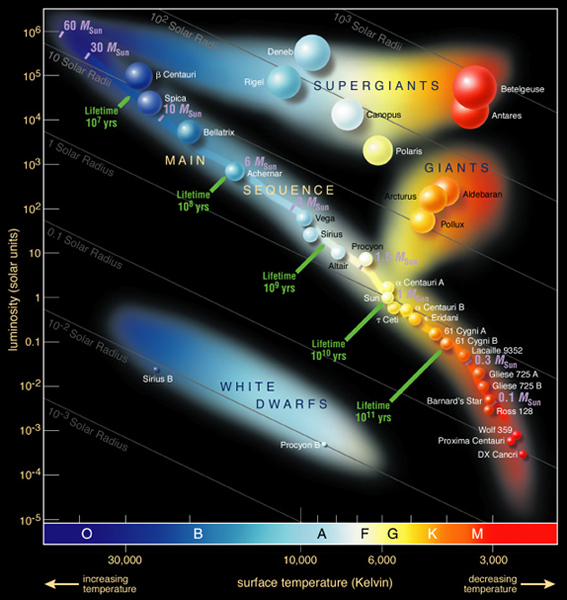
\includegraphics[scale=.30]{graphics/fig1}};
\end{tikzpicture}
\clearpage

%---------example slide----------------------------------------------------------
\section{Sometimes classification is surprisingly straightforward ...}

\begin{tikzpicture}[overlay]
  \node[anchor=south west] at (5,-3.5) {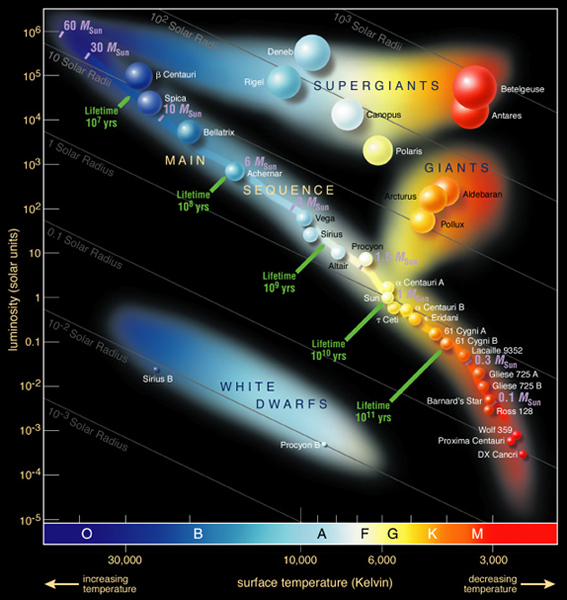
\includegraphics[scale=.30]{graphics/fig1}};
  \node[anchor=south west] at (0,-1)
  	{$\begin{aligned}
  	X &= (x_{1}, x_{2}, x_{3})\\
	C &= \{ c_1, c_2, c_3, c_4\} 
  	\end{aligned}$
  	};
 \end{tikzpicture}
\begin{textblock}{1}(0.505,.715)
  \footnotesize \texttt{Hertzsprung-Russell diagram}
 \end{textblock}
\clearpage




%---- insert complete .pdfs ---------------------
\usepackage{pdfpages}
\includepdf[pages={1-10}]{Experiment1b.pdf}

\includepdf[pages=1,scale=.8,pagecommand={\subsubsection*{Attachment 1: Using Git}},linktodoc=true]{graphics/Git1.pdf}
\includepdf[pages=2-,scale=.8,pagecommand={},linktodoc=true]{graphics/Git1.pdf}



%----size, resize, sizing .png and .jpeg ----------------------
	#.png file
\begin{figure}
	\includegraphics[scale = 0.25]{graphics/litrev2-ntb}
	\includegraphics[width=0.35\textwidth]{graphics/litrev2-ntb}
	\includegraphics[height=0.45\textwidth]{graphics/litrev2-ntb}
	
\end{figure}



% ---- size, resize, sizing .pdf and .eps ----------------------
	# .eps files
\begin{figure}
	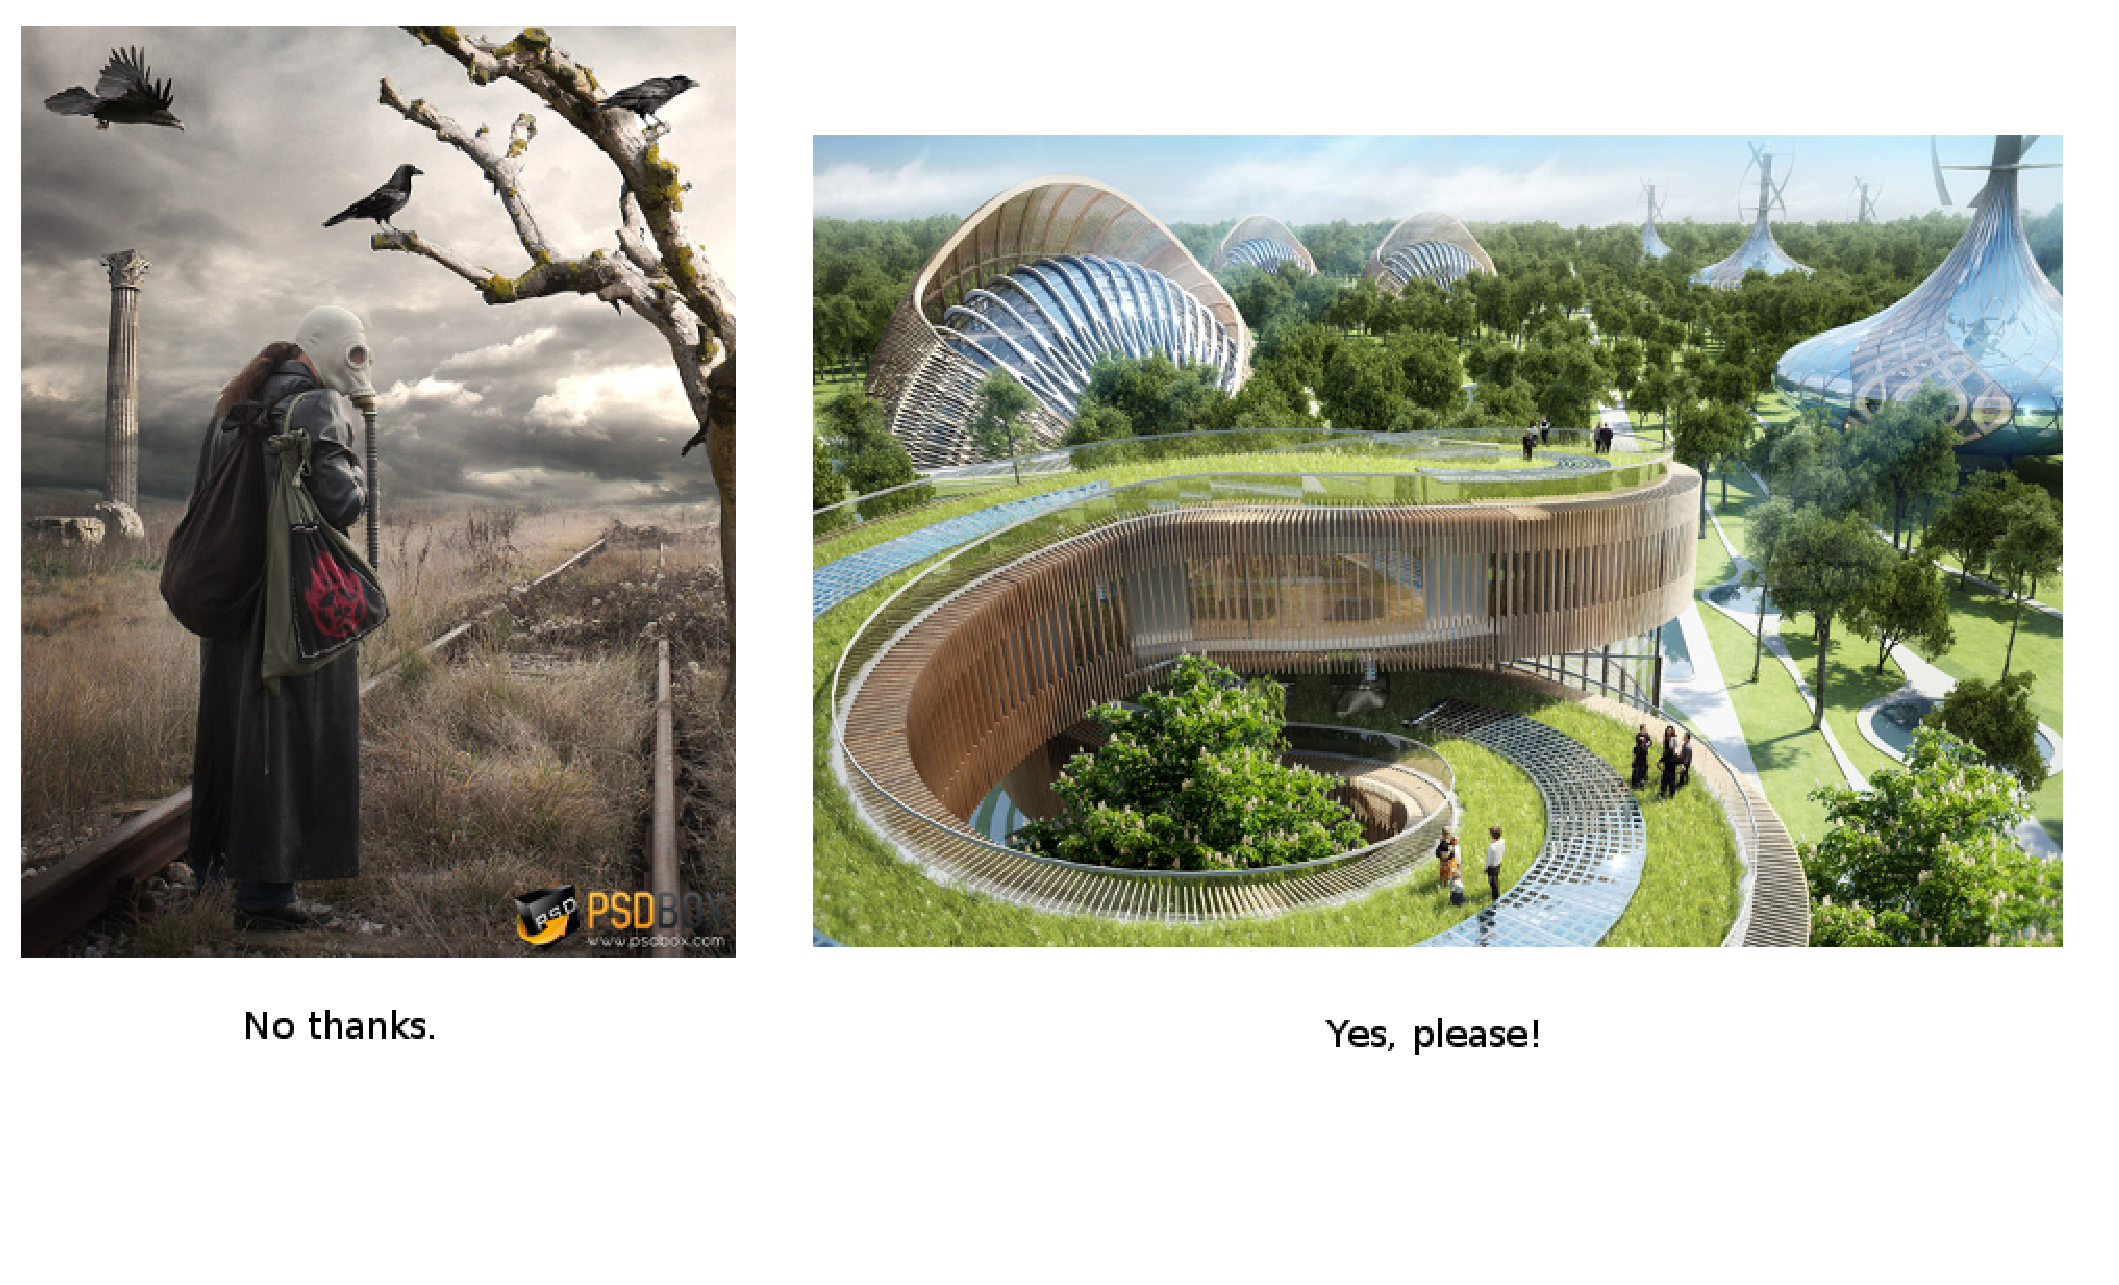
\includegraphics[width=20cm]{figs/Image1c}
\end{figure}

\begin{figure}
	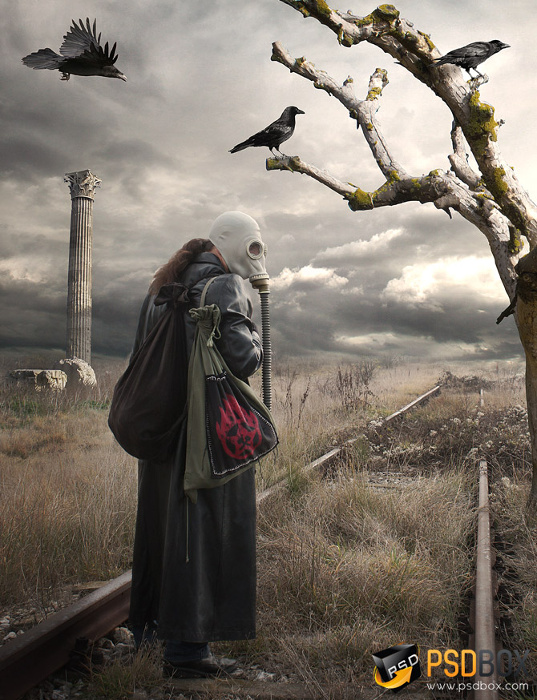
\includegraphics[height=15cm]{figs/Image2}
\end{figure}

	# .pdf files
\begin{figure}
    \includegraphics[width=1.0\textwidth, height=6 in, page=2]{/home/bmarron//Desktop/Problems1.pdf}
\end{figure}

\begin{figure}
	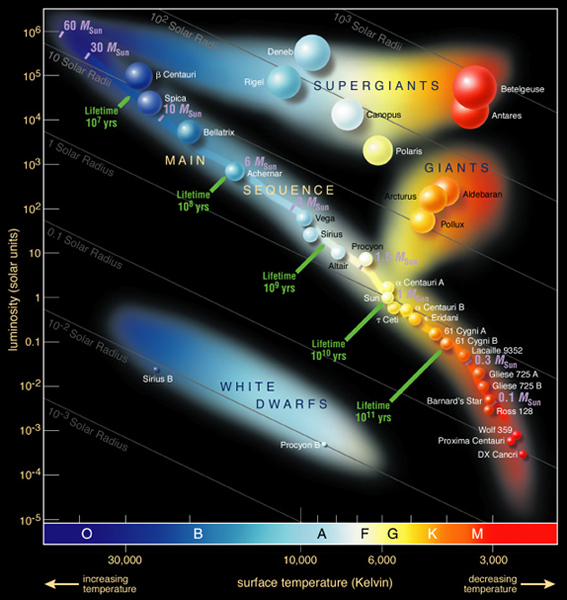
\includegraphics[width=0.35\textwidth, height=0.6\textheight]{graphics/fig1}
\end{figure}


%% --------- include attach pages .pdf ---------------------------------

If you're using Ubuntu 11.04 (or probably any Gnome distro) and can view the PDF in the built-in Document Viewer, you can then Print to file to save it as a PDF-1.5. (Save A Copy, in contrast, just creates a byte-identical copy of the file.

\usepackage{pdfpages}
 \includepdf[pages={1-10}]{Experiment1b.pdf}
 \includepdf[pages=-,pagecommand={},width=\textwidth]{graphics/IRSltr.pdf}
 
\includepdf[pages=1,scale=.8,pagecommand={\subsubsection*{Attachment 1: Using Git}\label{pdf:attachment1}},linktodoc=true]{myfile.pdf}
\includepdf[pages=2-,scale=.8,pagecommand={},linktodoc=true]{myfile.pdf}

\includepdf[pages=1,scale=.8,pagecommand={\subsubsection*{Attachment 1: Using Git}},linktodoc=true]{graphics/Git1.pdf}
\includepdf[pages=2-,scale=.8,pagecommand={},linktodoc=true]{graphics/Git1.pdf}




% ---- special indent paragraphs --------------------------

	#add this NOTE margin!!

     
     
     
% specialty commands
\newenvironment{myindentpar}[1]%
   {\begin{list}{}%
       {\setlength{\rightmargin}{#1}}%
           \item[]%
      }
     {\end{list}}
     
% To use
%\begin{myindentpar}{2em}
% blah blah blah
%\end {myindentpar}     

	#to use in doc
\begin{myindentpar}{1em}
text
\end{myindentpar}

\begin{myindentpar}{2em}
text
\end{myindentpar}

\begin{myindentpar}{3em}
text
\end{myindentpar}



% ---- big brackets --------------------------------------
 \left(  
 \right)
automatically expand to fit the material between them.


% ---- display fractions, ratios, division w/ larger num and denom ------------------
\newcommand\ddfrac[2]{\frac{\displaystyle #1}{\displaystyle #2}}
 $\ddfrac{TP+TN}{\Sigma Total Population}$

% ---- bars ------------------------------------
\usepackage{amsmath}

$\begin{array}{r}
a+b+c\\
a+b^3+c\\
a+\overline{b}+c\\
a+\overline{b}^3+c\\
a+\bar{b}+c\\
a+\bar{b}^3+c\\
a+\overline{b^3}+c\\
a+\bar{b^3}+c\\
a+b+c
\end{array}$


%------copy formulae from MathJax ----------------------
1. Show Math As ==> Original MathML
2. copy this to .txt file on Desktop
3. rename to math.xml file
4. run pandoc
%$ pandoc -f html+tex_math_dollars -t latex ~/Desktop/math.xml
 

%-------- copy formula from Wikipedia ---------------------
1. highlight 
2. Copy with "Outer HTML"




% ----summations -------------------------------------
\begin{align*}
  A &= \sum_{n=-\infty}^{+\infty} f(x) \\
%  B &= \smashoperator[r]{\sum_{n=-\infty}^{+\infty}} f(x) \\
%  C &= \sum_{\mathclap{n=-\infty}}^{+\infty} f(x) \\
  D &= \sum_{\substack{n={}\\-\infty}}^{+\infty} f(x) \\
  E &= \sum_{-\infty}^{\infty}\mathop{}_{\mkern-5mu n} f(x)
\end{align*}


%------------verbatim in Beamer slides----------------
%add fragile

\begin{frame}[fragile]\frametitle{}
Some prelim hypercycle data (package "

\small {
\begin{verbatim}
0,1.000000,1.000000,1.000000
1,1.981356,2.362799,1.736174
2,32.115404,46.416299,57.421630
3,257.593185,286.362595,451.561026
4,263.461357,262.878751,469.120181
5,275.632233,249.051347,470.750695
6,287.367319,244.186443,463.880935
7,294.987630,245.327804,455.133207
8,297.922755,249.185188,448.357092
9,297.505197,253.193102,444.779227
10,295.552920,255.961436,443.969766
11,293.481496,257.183393,444.820724
\end{verbatim}
}
\end{frame}



% -----verbatim text in math environment-----------------
\begin{equation*}
log \ (\verb!sed_n!) = \alpha + \beta_{1}\verb!slope! + \beta_{2}\verb!perc_ag! + \beta_{3}\verb!slope:perc_ag! + \varepsilon
\end{equation*}

%---- add a short verbatim ------------------------
\verb|this_tetxt|
\verb!Q1_part(a)_1.txt! 

%--- add verbatim text ------------------------------------
\verbatiminput{/home/bmarron//Desktop/PSU/PhD_EES/SoE/2016SoE010_GEOG694_Models/_PWFs_works_inprogress/Lab3/ascii_files_rgdal.txt}

%----------- add a verbatim block of text--------------------------
\begin{verbatim} 
to open the environment and to close it 
\end{verbatim}


%------verbatim in footnotes --------------------
http://tex.stackexchange.com/questions/203/how-to-obtain-verbatim-text-in-a-footnote

\usepackage{bigfoot}
\footnote{\verb|But, it does work!|}

%---- add trademark/registered copyright symbol ---------------------------
Netica\textsuperscript{\textregistered}
Upwork$^{\tiny{\textregistered}}$

%---- add watermark----------------------------
\usepackage{everypage}                                           % Required for watermarks
\usepackage{draftwatermark}
\SetWatermarkLightness{0.95}
\SetWatermarkScale{0.75}                                          % Set to 1.0 for default
\SetWatermarkText{FINAL DRAFT}                                    % comment out for default (DRAFT)   



%---- transposed matrix --------------------------
When there are N parameters, so that θ is a N × 1 vector 
\theta = \begin{bmatrix} \theta_{1}, \theta_{2}, \dots , \theta_{N} \end{bmatrix}^{\mathrm T}, 

%---- summations -----------------
$ \mathbf{\dot x} = (A_{i}Q_{i} - D_{i})x_{i} + \sum\limits_{k\neq i}^n w_{ik}x_{k} + \phi _{i} $

%--------cut and paste from Wikipedia--------------
$ {\left(\mathcal{I} \left(\theta \right) \right)}_{i, j} = \operatorname{E} \left[\left. \left(\frac{\partial}{\partial\theta_i} \log f(X;\theta)\right) \left(\frac{\partial}{\partial\theta_j} \log f(X;\theta)\right) \right|\theta\right] $



%-----------more tables ; center table------------------------------

\begin{table}[!htbp] \centering 
  \caption{Field characteristics of the Level3 formatted and pre-processed Metropolitan Family Service (MFS) dataset.} 
  \label{tab:bm1} 
\begin{tabular}{@{\extracolsep{5pt}}lcl} 
\toprule
Field & \multicolumn{1}{c}{Data Type} & \multicolumn{1}{l}{Values Range} \\
\midrule
School Name & Categorical & 0 - 22 \\
School District & Categorical & 0 - 4\\
School Type & Categorical & 0 - 2\\
Age	& Continuous & 6 - 22\\
Gender & Categorical & 0 - 3\\
Language & Categorical & 0 - 57\\
African	& Binary & 0 - 1\\
Asian & Binary & 0 - 1\\
Black/ African American	& Binary & 0 - 1\\
Latino/Hispanic	& Binary & 0 - 1\\
Middle Eastern	& Binary & 0 - 1\\
Native American/ Alaska Native	& Binary & 0 - 1\\
Native Hawaiian/ Pacific Islander & Binary & 0 - 1\\
Slavic & Binary & 0 - 1\\
White & Binary & 0 - 1\\
Declined & Binary & 0 - 1\\
Days Attended (Class attribute) & Binary & 0 - 1\\
\bottomrule
\end{tabular} 
\end{table}


\begin{table} \centering 
  \caption{Classification report of the MultinomialNB classifier applied to the test dataset. The test dataset was randomly selected from the Level4 formatted and pre-processed Metropolitan Family Service (MFS) dataset.} 
  \label{tab:bm3}
\begin{tabular}{lccc}
\toprule
Accuracy & Precision & Recall & F1 Score\\
\midrule
0.61 & 0.61 & 0.61 & 0.61 \\
\bottomrule
\end{tabular}
\end{table}




\begin{table} \centering 
  \caption{Confusion matrix of the MultinomialNB classifier applied to the test dataset. The test dataset was randomly selected from the Level4 formatted and pre-processed Metropolitan Family Service (MFS) dataset. The test dataset contained 1636 records.} 
  \label{tab:bm2} 
\begin{tabular}{lrr}
\toprule
{} &    1 &    0 \\
\midrule
1 &  463 &  273 \\
0 &  373 &  527 \\
\bottomrule
\end{tabular}
\end{table}



%---- table1 ----------------------------------
\begin{table}[!htbp] \centering 
  \caption{The MLEs and asymmetric, percentile-based bootstrap confidence intervals for transition matrix values b21 and b22 for the state-space model,\ \textit{process model3}.} 
  \label{} 
\begin{tabular}{@{\extracolsep{5pt}}lccc} 
\\[-1.8ex]\hline 
\hline \\[-1.8ex] 
Parameter & \multicolumn{1}{c}{True value} & \multicolumn{1}{c}{MLE} & \multicolumn{1}{c}{90\% CI} \\
\hline \\[-1.8ex]
b21 & -.25 & -.244 & [-.271, -.073]\\
b22 & 1.2 & 1.18 & [-.474, 1.76]\\
\hline \\[-1.8ex]
\end{tabular} 
\end{table}

%---- table2 --------------------------------------
\begin{table}[!htbp] \centering 
  \caption{The output statistics for three, forward addition variable selection procedures applied to the \texttt{creditscore.csv} dataset.} 
  \label{} 
\begin{tabular}{@{\extracolsep{5pt}}lccc} 
\\[-1.8ex]\hline 
\hline \\[-1.8ex] 
glm() & \multicolumn{1}{c}{F-ratio} & \multicolumn{1}{c}{AIC} & \multicolumn{1}{c}{BIC} \\ 
\hline \\[-1.8ex]
Intercept only & --- & 185.88 & 188.48 \\ 
Intercept + IV1 & 15.75 & 168.49 & 173.70 \\
Intercept + IV1 + IV2 & 3.95 & 165.78 & 173.59 \\
Intercept + IV1 + IV2 + IV3 & 3.55 & 163.67 & 174.09 \\
\hline \\[-1.8ex]
\footnotesize IV1 = Monthly.credit.card.exp\\
\footnotesize IV2 = Income.per.dependent\\
\footnotesize IV3 = Self.employed\\
\end{tabular} 
\end{table}

%---- longtable1; table across multiple pages -----------------------------------
\usepackage{longtable}
\begin{longtable}{cccc}
\caption{The 57 features used for the SVM in Experiment 2 ranked by the absolute value of their weight and the cumulative effect on the the SVM accuracy.} \\
[-1.8ex]\hline \hline \\[-1.8ex] 
 Weight Order  & Feature Number & SVM weight & Cumulative Accuracy \\
\hline \\[-1.8ex]
\endfirsthead

{\centering {\tablename\ \thetable{} -- continued from previous page}} \\
[1.8ex]\hline \hline \\[-1.8ex] 
 Weight Order  & Feature Number & SVM weight & Accuracy \\
\hline \\[-1.8ex]
\endhead

\multicolumn{4}{r}{{Continued on next page ...}} 
\endfoot

\hline 
\endlastfoot

1 & 26 & 2.4654 & 0.6098\\
2 & 24 & 1.4083 & 0.7339\\
3 & 30 & 1.4016 & 0.7356\\
4 & 52 & 1.1448 & 0.7582\\
5 & 45 & 0.9517 & 0.7864\\
6 & 6 & 0.8817 & 0.8366\\
7 & 15 & 0.8394 & 0.8664\\
8 & 44 & 0.7067 & 0.8758\\
9 & 25 & 0.6905 & 0.8780\\
10 & 40 & 0.6637 & 0.8813\\
11 & 41 & 0.6196 & 0.8940\\
12 & 34 & 0.5762 & 0.8945\\
13 & 4 & 0.4973 & 0.8984\\
14 & 23 & 0.4647 & 0.9045\\
15 & 55 & 0.3969 & 0.9161\\
16 & 22 & 0.3652 & 0.9177\\
17 & 53 & 0.3602 & 0.9210\\
18 & 38 & 0.3255 & 0.9210\\
19 & 3 & 0.3071 & 0.9227\\
20 & 28 & 0.2972 & 0.9227\\
21 & 16 & 0.2909 & 0.9199\\
22 & 7 & 0.2876 & 0.9194\\
23 & 43 & 0.2698 & 0.9199\\
24 & 54 & 0.2591 & 0.9194\\
25 & 14 & 0.2567 & 0.9194\\
26 & 32 & 0.2440 & 0.9194\\
27 & 51 & 0.2286 & 0.9183\\
28 & 56 & 0.2272 & 0.9216\\
29 & 29 & 0.2243 & 0.9232\\
30 & 20 & 0.2226 & 0.9227\\
31 & 21 & 0.2024 & 0.9221\\
32 & 27 & 0.1986 & 0.9221\\
33 & 31 & 0.1856 & 0.9210\\
34 & 18 & 0.1719 & 0.9216\\
35 & 48 & 0.1593 & 0.9238\\
36 & 8 & 0.1498 & 0.9282\\
37 & 2 & 0.1333 & 0.9177\\
38 & 10 & 0.1115 & 0.9216\\
39 & 47 & 0.1035 & 0.9216\\
40 & 17 & 0.1033 & 0.9183\\
41 & 9 & 0.0931 & 0.9210\\
42 & 19 & 0.0911 & 0.9216\\
43 & 0 & 0.0907 & 0.9249\\
44 & 39 & 0.0849 & 0.9249\\
45 & 33 & 0.0706 & 0.9249\\
46 & 42 & 0.0680 & 0.9254\\
47 & 46 & 0.0558 & 0.9232\\
48 & 5 & 0.0471 & 0.9260\\
49 & 37 & 0.0354 & 0.9249\\
50 & 11 & 0.0301 & 0.9243\\
51 & 13 & 0.0236 & 0.9277\\
52 & 12 & 0.0234 & 0.9277\\
53 & 35 & 0.0206 & 0.9260\\
54 & 36 & 0.0187 & 0.9266\\
55 & 49 & 0.0014 & 0.9266\\
56 & 1 & 0.0003 & 0.9266\\
57 & 50 & 0.00003 & 0.9266\\
\end{longtable}


%----- longtable2 table across multiple pages ------------------------
\begin{center}
\begin{longtable}{|l|l|l|}
\caption[Feasible triples for a highly variable Grid]{Feasible triples for 
highly variable Grid, MLMMH.} \label{grid_mlmmh} \\

\hline \multicolumn{1}{|c|}{\textbf{Time (s)}} & \multicolumn{1}{c|}{\textbf{Triple chosen}} & \multicolumn{1}{c|}{\textbf{Other feasible triples}} \\ \hline 
\endfirsthead

\multicolumn{3}{c}%
{{\bfseries \tablename\ \thetable{} -- continued from previous page}} \\
\hline \multicolumn{1}{|c|}{\textbf{Time (s)}} &
\multicolumn{1}{c|}{\textbf{Triple chosen}} &
\multicolumn{1}{c|}{\textbf{Other feasible triples}} \\ \hline 
\endhead

\hline \multicolumn{3}{|r|}{{Continued on next page}} \\ \hline
\endfoot

\hline \hline
\endlastfoot

0 & (1, 11, 13725) & (1, 12, 10980), (1, 13, 8235), (2, 2, 0), (3, 1, 0) \\
2745 & (1, 12, 10980) & (1, 13, 8235), (2, 2, 0), (2, 3, 0), (3, 1, 0) \\
5490 & (1, 12, 13725) & (2, 2, 2745), (2, 3, 0), (3, 1, 0) \\
8235 & (1, 12, 16470) & (1, 13, 13725), (2, 2, 2745), (2, 3, 0), (3, 1, 0) \\
10980 & (1, 12, 16470) & (1, 13, 13725), (2, 2, 2745), (2, 3, 0), (3, 1, 0) \\
13725 & (1, 12, 16470) & (1, 13, 13725), (2, 2, 2745), (2, 3, 0), (3, 1, 0) \\
16470 & (1, 13, 16470) & (2, 2, 2745), (2, 3, 0), (3, 1, 0) \\
19215 & (1, 12, 16470) & (1, 13, 13725), (2, 2, 2745), (2, 3, 0), (3, 1, 0) \\
21960 & (1, 12, 16470) & (1, 13, 13725), (2, 2, 2745), (2, 3, 0), (3, 1, 0) \\
24705 & (1, 12, 16470) & (1, 13, 13725), (2, 2, 2745), (2, 3, 0), (3, 1, 0) \\
27450 & (1, 12, 16470) & (1, 13, 13725), (2, 2, 2745), (2, 3, 0), (3, 1, 0) \\
30195 & (2, 2, 2745) & (2, 3, 0), (3, 1, 0) \\
32940 & (1, 13, 16470) & (2, 2, 2745), (2, 3, 0), (3, 1, 0) \\
35685 & (1, 13, 13725) & (2, 2, 2745), (2, 3, 0), (3, 1, 0) \\
38430 & (1, 13, 10980) & (2, 2, 2745), (2, 3, 0), (3, 1, 0) \\
41175 & (1, 12, 13725) & (1, 13, 10980), (2, 2, 2745), (2, 3, 0), (3, 1, 0) \\
43920 & (1, 13, 10980) & (2, 2, 2745), (2, 3, 0), (3, 1, 0) \\
46665 & (2, 2, 2745) & (2, 3, 0), (3, 1, 0) \\
49410 & (2, 2, 2745) & (2, 3, 0), (3, 1, 0) \\
52155 & (1, 12, 16470) & (1, 13, 13725), (2, 2, 2745), (2, 3, 0), (3, 1, 0) \\
54900 & (1, 13, 13725) & (2, 2, 2745), (2, 3, 0), (3, 1, 0) \\
57645 & (1, 13, 13725) & (2, 2, 2745), (2, 3, 0), (3, 1, 0) \\
60390 & (1, 12, 13725) & (2, 2, 2745), (2, 3, 0), (3, 1, 0) \\
63135 & (1, 13, 16470) & (2, 2, 2745), (2, 3, 0), (3, 1, 0) \\
65880 & (1, 13, 16470) & (2, 2, 2745), (2, 3, 0), (3, 1, 0) \\
68625 & (2, 2, 2745) & (2, 3, 0), (3, 1, 0) \\
71370 & (1, 13, 13725) & (2, 2, 2745), (2, 3, 0), (3, 1, 0) \\
74115 & (1, 12, 13725) & (2, 2, 2745), (2, 3, 0), (3, 1, 0) \\
76860 & (1, 13, 13725) & (2, 2, 2745), (2, 3, 0), (3, 1, 0) \\
79605 & (1, 13, 13725) & (2, 2, 2745), (2, 3, 0), (3, 1, 0) \\
82350 & (1, 12, 13725) & (2, 2, 2745), (2, 3, 0), (3, 1, 0) \\
85095 & (1, 12, 13725) & (1, 13, 10980), (2, 2, 2745), (2, 3, 0), (3, 1, 0) \\
87840 & (1, 13, 16470) & (2, 2, 2745), (2, 3, 0), (3, 1, 0) \\
90585 & (1, 13, 16470) & (2, 2, 2745), (2, 3, 0), (3, 1, 0) \\
93330 & (1, 13, 13725) & (2, 2, 2745), (2, 3, 0), (3, 1, 0) \\
96075 & (1, 13, 16470) & (2, 2, 2745), (2, 3, 0), (3, 1, 0) \\
98820 & (1, 13, 16470) & (2, 2, 2745), (2, 3, 0), (3, 1, 0) \\
101565 & (1, 13, 13725) & (2, 2, 2745), (2, 3, 0), (3, 1, 0) \\
104310 & (1, 13, 16470) & (2, 2, 2745), (2, 3, 0), (3, 1, 0) \\
107055 & (1, 13, 13725) & (2, 2, 2745), (2, 3, 0), (3, 1, 0) \\
109800 & (1, 13, 13725) & (2, 2, 2745), (2, 3, 0), (3, 1, 0) \\
112545 & (1, 12, 16470) & (1, 13, 13725), (2, 2, 2745), (2, 3, 0), (3, 1, 0) \\
115290 & (1, 13, 16470) & (2, 2, 2745), (2, 3, 0), (3, 1, 0) \\
118035 & (1, 13, 13725) & (2, 2, 2745), (2, 3, 0), (3, 1, 0) \\
120780 & (1, 13, 16470) & (2, 2, 2745), (2, 3, 0), (3, 1, 0) \\
123525 & (1, 13, 13725) & (2, 2, 2745), (2, 3, 0), (3, 1, 0) \\
126270 & (1, 12, 16470) & (1, 13, 13725), (2, 2, 2745), (2, 3, 0), (3, 1, 0) \\
129015 & (2, 2, 2745) & (2, 3, 0), (3, 1, 0) \\
131760 & (2, 2, 2745) & (2, 3, 0), (3, 1, 0) \\
134505 & (1, 13, 16470) & (2, 2, 2745), (2, 3, 0), (3, 1, 0) \\
137250 & (1, 13, 13725) & (2, 2, 2745), (2, 3, 0), (3, 1, 0) \\
139995 & (2, 2, 2745) & (2, 3, 0), (3, 1, 0) \\
142740 & (2, 2, 2745) & (2, 3, 0), (3, 1, 0) \\
145485 & (1, 12, 16470) & (1, 13, 13725), (2, 2, 2745), (2, 3, 0), (3, 1, 0) \\
148230 & (2, 2, 2745) & (2, 3, 0), (3, 1, 0) \\
150975 & (1, 13, 16470) & (2, 2, 2745), (2, 3, 0), (3, 1, 0) \\
153720 & (1, 12, 13725) & (2, 2, 2745), (2, 3, 0), (3, 1, 0) \\
156465 & (1, 13, 13725) & (2, 2, 2745), (2, 3, 0), (3, 1, 0) \\
159210 & (1, 13, 13725) & (2, 2, 2745), (2, 3, 0), (3, 1, 0) \\
161955 & (1, 13, 16470) & (2, 2, 2745), (2, 3, 0), (3, 1, 0) \\
164700 & (1, 13, 13725) & (2, 2, 2745), (2, 3, 0), (3, 1, 0) \\
\end{longtable}
\end{center}

%-----another table ----------------------

\begin{table}[H]
\caption{Example table}
\centering
\begin{tabular}{llr}
\toprule
\multicolumn{2}{c}{Name} \\
\cmidrule(r){1-2}
First name & Last Name & Grade \\
\midrule
John & Doe & $7.5$ \\
Richard & Miles & $2$ \\
\bottomrule
\end{tabular}
\end{table}


%-------- table (threeparttable) footnotes -------------------------------------------------
 \begin{table}
\footnotesize
  \begin{threeparttable}[b]
    \caption{SWAT inputs categorized by modeling tasks and processes.}
      \label{tab:bm1}
      \centering      
    \begin{tabular}{llll}
    \hline \hline \\[-1.8ex]
    Task & Process & Input Category & Input \\
    \hline \\[-1.8ex]
    Watershed &&&\\
    Delineation & & & \\
    & Project Goals &&\\
    && Project Extent &\\
    & & & drainage area\tnote{1}\\
    Watershed &&&\\
    Subdivision & & & \\
    & Discretization & & \\
    && Subbasins and HRUs &\\
    & & & subbasins\tnote{4}\\
	& & & subbasin channels (main and tributary)\tnote{4}\\
	& & & hydrologic response units (HRUs)\tnote{4}\\
	&&& --- \\
	& & & digital elevation model (DEM; vector)\tnote{1}\\
	& & & land use land cover codes (raster)\tnote{2}\\
	& & & soil codes (vector)\tnote{2}\\
	&&& climate data \\
	Watershed & & &\\
    Simulation &&&\\
    & Routing Phase Hydrology &&\\
	&& Main Channel Routing & \\
	&&& water (variable storage coefficient method)\tnote{4}\\
	&&& sediments (stream power as fxn of peak channel velocity)\tnote{4}\\
	&&& nutrients (QUAL2E)\tnote{4}\\
	&&& pesticides (first-order decay relationships)\tnote{4}\\
	& & Reservoir Routing &\\
	&&& outflow\tnote{3}\\
	&&& sediments\tnote{4}\\
	&&& nutrients\tnote{4}\\
	&&& pesticides\tnote{4}\\
	\hline \\[-1.8ex]
    \end{tabular}
    \begin{tablenotes}
    \footnotesize 
    \item [1] User provided
    \item [2] User provided $\arrowvert$ from external databases $\arrowvert$ provided or calculated by SWAT
    \item [3] User provided $\arrowvert$ provided or calculated by SWAT
    \item [4] Calculated by SWAT
    \end{tablenotes}
  \end{threeparttable}
\end{table}





%---- bibliography at end of doc --------------------------------------
\renewcommand{\refname}{\large \textbf{References}} 
\bibliographystyle{/usr/local/share/texmf/tex/latex/apacite/apacite}
\bibliography{/home/bmarron//Desktop/BibTex/MyLibrary20151104}
\end{document}
